\documentclass[aspectratio=169, 10pt]{beamer}

% ── Packages ────────────────────────────────────────────────────────────────
\usepackage[utf8]{inputenc}
\usepackage[T1]{fontenc}
\usepackage{lmodern}
\usepackage{amsmath, amssymb, bm}
\usepackage{booktabs}
\usepackage{graphicx}
\usepackage{tikz}
\usepackage{xcolor}
\usepackage{hyperref}
\usepackage{pgfplots}
\pgfplotsset{compat=1.18}
\usetikzlibrary{arrows.meta, positioning, shapes.geometric, fit, backgrounds, calc}

% ── Color palette ───────────────────────────────────────────────────────────
\definecolor{spaceblue}{HTML}{0D1B2A}
\definecolor{teal}{HTML}{1F7A8C}
\definecolor{cyan}{HTML}{22B8CF}
\definecolor{silver}{HTML}{C8D6E5}
\definecolor{gold}{HTML}{F4C430}
\definecolor{alertred}{HTML}{E74C3C}
\definecolor{successgreen}{HTML}{2ECC71}

% ── Beamer theme ────────────────────────────────────────────────────────────
\usetheme{default}
\usecolortheme{default}
\setbeamercolor{normal text}{fg=silver, bg=spaceblue}
\setbeamercolor{frametitle}{fg=cyan, bg=spaceblue}
\setbeamercolor{title}{fg=white, bg=spaceblue}
\setbeamercolor{subtitle}{fg=silver}
\setbeamercolor{author}{fg=cyan}
\setbeamercolor{date}{fg=silver}
\setbeamercolor{institute}{fg=silver}
\setbeamercolor{structure}{fg=cyan}
\setbeamercolor{block title}{fg=white, bg=teal}
\setbeamercolor{block body}{fg=silver, bg=spaceblue!80}
\setbeamercolor{alerted text}{fg=gold}
\setbeamercolor{item}{fg=cyan}
\setbeamercolor{subitem}{fg=silver}
\setbeamercolor{footline}{fg=silver!60, bg=spaceblue}
\setbeamercolor{palette primary}{bg=teal, fg=white}

% ── Fonts ───────────────────────────────────────────────────────────────────
\setbeamerfont{title}{size=\Large, series=\bfseries}
\setbeamerfont{frametitle}{size=\large, series=\bfseries}
\setbeamerfont{block title}{series=\bfseries}

% ── Frame title with bottom rule ────────────────────────────────────────────
\setbeamertemplate{frametitle}{
  \vspace{0.3em}
  \textbf{\insertframetitle}\\[-0.1em]
  {\color{teal}\rule{\textwidth}{0.4pt}}
  \vspace{0.1em}
}

% ── Footer ──────────────────────────────────────────────────────────────────
\setbeamertemplate{footline}{
  \begin{beamercolorbox}[wd=\textwidth, ht=2.2ex, dp=1ex]{footline}
    \hspace{0.8em}
    {\scriptsize Galardi \& Vagnoli \hfill
     Deep SARSA vs Actor-Critic --- LunarLander-v3 \hfill
     \insertframenumber{} / \inserttotalframenumber\hspace{0.8em}}
  \end{beamercolorbox}
}
\setbeamertemplate{navigation symbols}{}
\setbeamertemplate{itemize item}{\color{cyan}$\bullet$}
\setbeamertemplate{itemize subitem}{\color{silver}$\circ$}

% ── Custom commands ──────────────────────────────────────────────────────────
\newcommand{\highlight}[1]{{\color{gold}\textbf{#1}}}
\newcommand{\keyword}[1]{{\color{cyan}\textit{#1}}}
\newcommand{\code}[1]{{\color{silver}\texttt{\small #1}}}

% ─────────────────────────────────────────────────────────────────────────────
%  METADATA
% ─────────────────────────────────────────────────────────────────────────────
\title{Deep SARSA vs Advantage Actor-Critic}
\subtitle{A Comparative Study on LunarLander-v3}
\author{Francesco Galardi \quad Andrea Vagnoli}
\institute{%
  Symbolic and Evolutionary Artificial Intelligence\\
  University of Pisa --- AIDE Master's Programme, 2025/2026}
\date{June 2026}

% ══════════════════════════════════════════════════════════════════════════════
\begin{document}
% ══════════════════════════════════════════════════════════════════════════════

% ─────────────────────────────────────────────────────────────────────────────
%  SLIDE 1 — TITLE
% ─────────────────────────────────────────────────────────────────────────────
{
\setbeamertemplate{footline}{}
\begin{frame}[plain]
  \begin{tikzpicture}[remember picture, overlay]
    \fill[spaceblue] (current page.south west) rectangle (current page.north east);
    \foreach \x/\y in {0.1/0.9, 0.3/0.2, 0.7/0.8, 0.9/0.1, 0.5/0.5,
                        0.15/0.6, 0.85/0.4, 0.4/0.95, 0.6/0.05, 0.2/0.75}
      \fill[white, opacity=0.6] ($(current page.south west)+(\x\textwidth,\y\textheight)$)
            circle (0.8pt);
    \draw[teal, line width=1pt]
      ($(current page.west)+(0,-0.05\textheight)$) -- ($(current page.east)+(0,-0.05\textheight)$);
  \end{tikzpicture}

  \vspace{2em}
  \begin{center}
    {\color{cyan}\Large\textbf{Deep SARSA vs Advantage Actor-Critic}}\\[0.4em]
    {\color{silver}\large A Comparative Study on LunarLander-v3}\\[1.2em]
    {\color{teal}\rule{0.5\textwidth}{0.4pt}}\\[0.8em]
    {\color{silver}Francesco Galardi \quad $\cdot$ \quad Andrea Vagnoli}\\[0.3em]
    {\color{silver!60}\small Symbolic and Evolutionary Artificial Intelligence}\\
    {\color{silver!60}\small University of Pisa --- AIDE Master's Programme}\\[0.4em]
    {\color{silver!60}\small June 2026}
  \end{center}
\end{frame}
}

% ─────────────────────────────────────────────────────────────────────────────
%  SLIDE 2 — OUTLINE
% ─────────────────────────────────────────────────────────────────────────────
\begin{frame}{Outline}
  \begin{columns}[T]
    \column{0.48\textwidth}
      \begin{block}{Environment \& MDP}
        \begin{itemize}
          \item LunarLander-v3 overview
          \item State \& Action spaces
          \item Reward function \& stochasticity
        \end{itemize}
      \end{block}
      \vspace{0.5em}
      \begin{block}{Algorithms}
        \begin{itemize}
          \item SARSA: theory \& neural extension
          \item Actor-Critic (A2C): theory \& design
          \item Side-by-side comparison
        \end{itemize}
      \end{block}
    \column{0.48\textwidth}
      \begin{block}{Implementation}
        \begin{itemize}
          \item Network architecture
          \item Training setup \& hyperparameters
          \item Exploration strategies
        \end{itemize}
      \end{block}
      \vspace{0.5em}
      \begin{block}{Results}
        \begin{itemize}
          \item Learning curves (mean $\pm$ 95\% CI)
          \item Statistical significance (Welch's $t$-test)
          \item Efficiency, generalisation, failure analysis
        \end{itemize}
      \end{block}
  \end{columns}
\end{frame}

% ─────────────────────────────────────────────────────────────────────────────
%  SLIDE 3 — ENVIRONMENT OVERVIEW
% ─────────────────────────────────────────────────────────────────────────────
\begin{frame}{The LunarLander-v3 Environment}
  \begin{columns}[T]
    \column{0.55\textwidth}
      \textbf{Setting}: A rocket must land safely between two flags.\\[0.6em]
      \begin{itemize}
        \item Simulates realistic gravitational physics
        \item Main engine + two lateral thrusters
        \item Episode ends on landing, crash, or out-of-bounds
        \item \highlight{Solved} when mean reward $\geq 200$ over 100 episodes
      \end{itemize}
      \vspace{0.6em}
      \begin{block}{Why LunarLander-v3?}
        \begin{itemize}
          \item \textbf{Continuous state, discrete actions}: ideal for
                comparing value-based vs.\ policy-gradient methods
          \item Well-known benchmark with clear success criterion
          \item Supports wind / turbulence for generalisation tests
        \end{itemize}
      \end{block}
    \column{0.42\textwidth}
      
\begin{tikzpicture}
        \fill[spaceblue!50] (0,0) rectangle (4.5,4);
        \fill[teal!30] (0,0) rectangle (4.5,0.4);
        \draw[gold, line width=1.2pt] (1.0,0.4) -- (1.0,1.2);
        \draw[gold, fill=gold!80] (1.0,1.2) -- (1.4,1.0) -- (1.0,0.8) -- cycle;
        \draw[gold, line width=1.2pt] (3.5,0.4) -- (3.5,1.2);
        \draw[gold, fill=gold!80] (3.5,1.2) -- (3.9,1.0) -- (3.5,0.8) -- cycle;
        \fill[silver] (2.0,2.8) -- (2.5,2.8) -- (2.6,2.5) -- (2.5,2.2)
                       -- (2.0,2.2) -- (1.9,2.5) -- cycle;
        \fill[cyan!60] (2.1,2.55) rectangle (2.4,2.8);
        \draw[silver, line width=1.2pt] (1.9,2.3) -- (1.5,1.9);
        \draw[silver, line width=1.2pt] (2.6,2.3) -- (3.0,1.9);
        \fill[gold, opacity=0.8] (2.15,2.2) -- (2.35,2.2) -- (2.25,1.75) -- cycle;
        \fill[alertred, opacity=0.5] (2.2,2.2) -- (2.3,2.2) -- (2.25,2.0) -- cycle;
        \foreach \x/\y in {0.3/3.5, 0.8/3.2, 1.5/3.7, 3.0/3.5, 4.0/3.2, 4.2/3.8}
          \fill[white, opacity=0.7] (\x,\y) circle (1pt);
        \node[color=silver, font=\tiny] at (2.25,0.2) {Landing Zone};
      \end{tikzpicture}
  \end{columns}
\end{frame}

% ─────────────────────────────────────────────────────────────────────────────
%  SLIDE 4 — MDP: STATE & ACTION SPACE
% ─────────────────────────────────────────────────────────────────────────────
\begin{frame}{MDP Formulation: State \& Action Space}
  \begin{columns}[T]
    \column{0.50\textwidth}
      \begin{block}{State Space $\mathcal{S} \subset \mathbb{R}^8$}
        \vspace{0.3em}
        \small
        \begin{tabular}{lll}
          \toprule
          \textbf{Index} & \textbf{Feature} & \textbf{Range}\\
          \midrule
          $s_0$ & $x$ position     & $[-1.5, +1.5]$\\
          $s_1$ & $y$ position     & $[0, +1.5]$\\
          $s_2$ & $x$ velocity     & $\mathbb{R}$\\
          $s_3$ & $y$ velocity     & $\mathbb{R}$\\
          $s_4$ & angle $\theta$   & $[-\pi, +\pi]$\\
          $s_5$ & angular velocity & $\mathbb{R}$\\
          $s_6$ & left leg contact & $\{0, 1\}$\\
          $s_7$ & right leg contact& $\{0, 1\}$\\
          \bottomrule
        \end{tabular}
        \vspace{0.3em}
      \end{block}
      \textbf{Normalisation}: running mean/std (Welford) applied
      per-observation to keep inputs well-conditioned for both networks.
    \column{0.46\textwidth}
      \begin{block}{Action Space $\mathcal{A}$ --- Discrete(4)}
        \vspace{0.3em}
        \begin{tabular}{ll}
          \toprule
          \textbf{Action} & \textbf{Effect}\\
          \midrule
          0 & Do nothing\\
          1 & Fire left thruster\\
          2 & Fire main engine\\
          3 & Fire right thruster\\
          \bottomrule
        \end{tabular}
      \end{block}
      \vspace{0.5em}
      \begin{alertblock}{Impact on algorithm choice}
        Discrete actions allow \textbf{Deep SARSA} to output Q-values
        for all 4 actions in one forward pass, and allow \textbf{A2C}
        to use a \keyword{Categorical} distribution with clean entropy
        computation $H = -\sum_a \pi \log \pi$.
      \end{alertblock}
  \end{columns}
\end{frame}

% ─────────────────────────────────────────────────────────────────────────────
%  SLIDE 5 — MDP: REWARD & STOCHASTICITY
% ─────────────────────────────────────────────────────────────────────────────
\begin{frame}{MDP Formulation: Reward \& Stochasticity}
  \begin{columns}[T]
    \column{0.52\textwidth}
      \begin{block}{Reward Function (Dense)}
        Per-step shaping reward:
        \[
          r_t = \underbrace{-\Delta d}_{\text{approach}} +
                \underbrace{-0.03|v|}_{\text{velocity pen.}} +
                \underbrace{-0.3|\omega|}_{\text{rotation}} +
                \underbrace{0.1 \cdot (\ell_L + \ell_R)}_{\text{leg contacts}}
        \]
        Plus terminal bonuses:
        \begin{itemize}
          \item $+100$ for a successful landing
          \item $-100$ for crash or boundary exit
          \item $-0.3$ per engine firing (fuel cost)
        \end{itemize}
      \end{block}
      \textbf{Dense reward}: feedback at every step reduces the credit
      assignment problem compared to sparse alternatives.
    \column{0.44\textwidth}
      \begin{block}{Stochasticity Sources}
        \begin{itemize}
          \item \textbf{Initial conditions}: position and velocity
                sampled from a bounded uniform distribution
          \item \textbf{Optional wind}: $\mathcal{N}(0, \sigma_w^2)$
                lateral force added each step
          \item \textbf{Turbulence}: random torque
                $\mathcal{N}(0, \sigma_T^2)$
        \end{itemize}
      \end{block}
      \vspace{0.4em}
      \begin{alertblock}{Reward hacking risk}
        Agent may learn to \emph{hover} without landing to avoid the
        crash penalty. Monitored via episode length and leg-contact
        rate during evaluation.
      \end{alertblock}
  \end{columns}
\end{frame}

% ─────────────────────────────────────────────────────────────────────────────
%  SLIDE 6 — SARSA: THEORY
% ─────────────────────────────────────────────────────────────────────────────
\begin{frame}{Algorithm 1: SARSA --- Theory}
  \begin{columns}[T]
    \column{0.50\textwidth}
      \textbf{SARSA} (Sutton \& Barto, 2018, \S6.4) is a model-free,
      \keyword{on-policy} TD control algorithm.\\[0.5em]

      At each step the agent uses the tuple
      $(s_t, a_t, r_t, s_{t+1}, a_{t+1})$ to update:

      \[
        \boxed{Q(s_t, a_t) \leftarrow Q(s_t, a_t) +
               \alpha \bigl[r_t + \gamma Q(s_{t+1}, a_{t+1}) -
               Q(s_t, a_t)\bigr]}
      \]

      \begin{itemize}
        \item $a_{t+1}$ is sampled from the \textbf{current policy}
              ($\varepsilon$-greedy) --- not from $\max_{a'}$
        \item This makes the method \textbf{on-policy}: the target
              includes the next action actually taken
        \item Converges to the optimal policy under mild conditions
      \end{itemize}
    \column{0.46\textwidth}
      \begin{block}{SARSA vs Q-Learning}
        \vspace{0.3em}
        \begin{tabular}{lcc}
          \toprule
          & \textbf{SARSA} & \textbf{Q-Learning}\\
          \midrule
          Target & $Q(s', a')$ & $\max_{a'}Q(s',a')$\\
          Policy & on-policy & off-policy\\
          Safety & safer & riskier\\
          \bottomrule
        \end{tabular}
      \end{block}
      \vspace{0.5em}
      \begin{block}{Key intuition}
        SARSA is \emph{pessimistic}: it evaluates the policy it
        actually follows, including exploration mistakes. This
        yields more \textbf{conservative} policies in stochastic
        environments.
      \end{block}
  \end{columns}
\end{frame}

% ─────────────────────────────────────────────────────────────────────────────
%  SLIDE 7 — DEEP SARSA
% ─────────────────────────────────────────────────────────────────────────────
\begin{frame}{Deep SARSA: Neural Network Extension}
  \begin{columns}[T]
    \column{0.50\textwidth}
      Tabular SARSA cannot handle the continuous state space
      ($\mathcal{S} \subset \mathbb{R}^8$). We replace the Q-table
      with a neural network $Q_\theta(s, \cdot)$: one forward pass
      yields Q-values for \emph{all} 4 actions simultaneously.\\[0.4em]

      \textbf{Loss function:}
      \[
        \mathcal{L}(\theta) =
        \bigl(Q_\theta(s,a) -
        \underbrace{[r + \gamma Q_{\theta^-}(s', a')]}_{\text{SARSA target}}\bigr)^2
      \]
      where $\theta^-$ are the \keyword{target network} parameters
      (lagged copy, synced every 25 episodes).

    \column{0.46\textwidth}
      \begin{block}{Extensions over base codebase}
        \begin{itemize}
          \item \textbf{Target network}: stabilises the Bellman
                target, preventing oscillations (Mnih et al., 2015).
                Synced every 25 episodes.
          \item \textbf{Short-horizon replay buffer} (50\,k): de-correlates
                consecutive gradient updates while staying
                \emph{approximately} on-policy (stores $a'$ alongside
                each transition)
          \item \textbf{Gradient clipping} ($\|\nabla\| \leq 10$)
                for stability in early training
        \end{itemize}
      \end{block}
      \vspace{0.3em}
      \begin{alertblock}{On-policy integrity}
        Each stored transition also saves $a'$ (sampled from the
        \emph{current} $\varepsilon$-greedy policy), preserving exact
        SARSA semantics inside the replay buffer.
      \end{alertblock}
  \end{columns}
\end{frame}

% ─────────────────────────────────────────────────────────────────────────────
%  SLIDE 8 — A2C: THEORY
% ─────────────────────────────────────────────────────────────────────────────
\begin{frame}{Algorithm 2: Advantage Actor-Critic (A2C) --- Theory}
  \begin{columns}[T]
    \column{0.50\textwidth}
      A2C is a synchronous \keyword{policy-gradient} method
      (Mnih et al., 2016) combining:

      \begin{itemize}
        \item \textbf{Actor} $\pi_\theta(a|s)$: stochastic policy
        \item \textbf{Critic} $V_w(s)$: state-value baseline
      \end{itemize}

      \vspace{0.4em}
      \textbf{Actor gradient} (REINFORCE with baseline):
      \[
        \nabla_\theta J = \mathbb{E}\bigl[
          \nabla_\theta \log \pi_\theta(a|s) \cdot A(s,a)
        \bigr]
      \]

      \textbf{$n$-step advantage} ($n=200$, near-Monte Carlo):
      \[
        A_t = \sum_{k=0}^{n-1}\gamma^k r_{t+k} +
              \gamma^n V_w(s_{t+n}) - V_w(s_t)
      \]

      \textbf{Critic loss}:
      $\mathcal{L}_c = \bigl(G_t - V_w(s_t)\bigr)^2$

    \column{0.46\textwidth}
      \begin{block}{Entropy regularisation}
        \[
          \mathcal{L}_\pi = -\log \pi_\theta(a|s) \cdot A_t
                            - \beta H[\pi_\theta(\cdot|s)]
        \]
        The entropy bonus $\beta H[\pi]$ prevents premature
        convergence to deterministic (brittle) policies.
        Final value: $\beta = 0.001$.
      \end{block}
      \vspace{0.4em}
      \begin{block}{Why A2C over plain REINFORCE?}
        \begin{itemize}
          \item Critic reduces gradient variance via the baseline
          \item $n$-step returns balance bias--variance trade-off
          \item No replay buffer needed: fully on-policy
        \end{itemize}
      \end{block}
  \end{columns}
\end{frame}

% ─────────────────────────────────────────────────────────────────────────────
%  SLIDE 9 — ALGORITHM COMPARISON
% ─────────────────────────────────────────────────────────────────────────────
\begin{frame}{Algorithm Comparison}
  \begin{center}
  \renewcommand{\arraystretch}{1.35}
  \begin{tabular}{lcc}
    \toprule
    \textbf{Property} & \textbf{Deep SARSA} & \textbf{A2C} \\
    \midrule
    Paradigm          & Value-based (TD)   & Policy gradient \\
    Policy type       & Implicit ($\varepsilon$-greedy on $Q$) & Explicit ($\pi_\theta$) \\
    On/Off policy     & On-policy          & On-policy \\
    Exploration       & $\varepsilon$-greedy & Entropy bonus $\beta H[\pi]$ \\
    Replay buffer     & Yes (50\,k, semi-on-policy) & No \\
    Target network    & Yes (sync every 25 ep) & No \\
    Networks          & 1 Q-network + target & Actor + Critic (separate LR) \\
    Update frequency  & Per mini-batch (batch=64) & Every $n=200$ steps \\
    Training budget   & 2\,000 episodes    & 5\,000 episodes \\
    \bottomrule
  \end{tabular}
  \end{center}
  \vspace{0.3em}
  \begin{columns}
    \column{0.48\textwidth}
      \begin{block}{\color{white}SARSA advantage}
        More stable and sample-efficient; all 5 seeds converge
        between episodes 1050--1250.
      \end{block}
    \column{0.48\textwidth}
      \begin{block}{\color{white}A2C advantage}
        Stochastic policy with entropy regularisation yields
        far better zero-shot generalisation to harder variants.
      \end{block}
  \end{columns}
\end{frame}

% ─────────────────────────────────────────────────────────────────────────────
%  SLIDE 10 — NETWORK ARCHITECTURE
% ─────────────────────────────────────────────────────────────────────────────
\begin{frame}{Neural Network Architecture}
  \begin{columns}[T]
    \column{0.50\textwidth}
      \textbf{Deep SARSA} --- single Q-network (+ frozen target copy):
      \[
        \mathbb{R}^8 \xrightarrow{\text{FC-256}} \text{ReLU}
        \xrightarrow{\text{FC-256}} \text{ReLU}
        \xrightarrow{\text{FC-4}} \mathbb{R}^4
      \]
      Output: $Q(s, a)$ for each of the 4 actions.\\[0.8em]
      \textbf{A2C} --- two separate networks:
      \[
        \underbrace{\mathbb{R}^8 \!\to\! 256 \!\to\! 256 \!\to\! 4}_{\text{Actor}: \text{Softmax} \Rightarrow \pi_\theta(a|s)}
        \quad
        \underbrace{\mathbb{R}^8 \!\to\! 256 \!\to\! 256 \!\to\! 1}_{\text{Critic}: V_w(s)}
      \]
    \column{0.46\textwidth}
      \begin{block}{Design choices}
        \begin{itemize}
          \item \textbf{Width 256}: matches RL Baselines3 Zoo tuned
                architecture for LunarLander-v3 (Raffin et al., 2021)
          \item \textbf{ReLU}: avoids vanishing gradients; standard
                for discrete-action control tasks
          \item \textbf{Separate actor/critic}: independent learning
                rates ($\alpha_\pi = 3{\times}10^{-4}$,
                $\alpha_V = 10^{-4}$) reduce the risk of the critic
                destabilising the actor
          \item \textbf{Gradient clipping}: $\|\nabla\| \leq 10$
                (SARSA Q-net), $\|\nabla\| \leq 0.5$ (A2C actor \& critic)
        \end{itemize}
      \end{block}
  \end{columns}
\end{frame}

% ─────────────────────────────────────────────────────────────────────────────
%  SLIDE 11 — TRAINING SETUP & HYPERPARAMETERS
% ─────────────────────────────────────────────────────────────────────────────
\begin{frame}{Training Setup \& Hyperparameters}
  \begin{columns}[T]
    \column{0.48\textwidth}
      \begin{block}{Deep SARSA \small(2\,000 episodes)}
        \vspace{0.2em}
        \small
        \begin{tabular}{ll}
          \toprule
          \textbf{Parameter} & \textbf{Value} \\
          \midrule
          Learning rate $\alpha$   & $3\times 10^{-4}$ \\
          Discount $\gamma$        & $0.99$ \\
          $\varepsilon_0 \to \varepsilon_\infty$ & $1.0 \to 0.01$ \\
          $\varepsilon$ decay      & $0.9975$ / ep\\
          Target sync freq.        & $25$ episodes \\
          Batch size               & $64$ \\
          Buffer capacity          & $50{,}000$ \\
          \bottomrule
        \end{tabular}
      \end{block}
    \column{0.48\textwidth}
      \begin{block}{Actor-Critic A2C \small(5\,000 episodes)}
        \vspace{0.2em}
        \small
        \begin{tabular}{ll}
          \toprule
          \textbf{Parameter} & \textbf{Value}\\
          \midrule
          Actor LR $\alpha_\pi$    & $3\times 10^{-4}$ \\
          Critic LR $\alpha_V$     & $1\times 10^{-4}$ \\
          Discount $\gamma$        & $0.99$ \\
          Entropy coef $\beta$     & $0.001$ \\
          $n$-step horizon         & $200$ \\
          Grad clip (actor/critic) & $0.5$ \\
          \bottomrule
        \end{tabular}
      \end{block}
  \end{columns}
  \vspace{0.3em}
  \begin{block}{Common setup \& hyperparameter source}
    \textbf{5 seeds} $\{42, 123, 456, 789, 1234\}$, observation normalisation (Welford).
    Initial values from \textbf{RL Baselines3 Zoo} (Raffin et al., 2021) --- Optuna-tuned
    on LunarLander-v3. Final values adjusted from training logs
    (buffer $10\text{k}{\to}50\text{k}$; $\beta\;0.05{\to}0.001$; $n_\text{steps}\;5{\to}200$).
  \end{block}
\end{frame}

% ─────────────────────────────────────────────────────────────────────────────
%  SLIDE 12 — EXPLORATION
% ─────────────────────────────────────────────────────────────────────────────
\begin{frame}{Exploration--Exploitation Trade-off}
  \begin{columns}[T]
    \column{0.50\textwidth}
      \begin{block}{Deep SARSA --- $\varepsilon$-greedy}
        \[
          \pi(a|s) = \begin{cases}
            \text{Uniform}(\mathcal{A}) & \text{w.p. } \varepsilon_t\\
            \arg\max_a Q_\theta(s,a)    & \text{w.p. } 1-\varepsilon_t
          \end{cases}
        \]
        $\varepsilon_t = \max(0.01,\ 0.9975^t)$.
        Reaches 0.01 at ep\,$\approx\!1840$\\
        (from $0.9975^n = 0.01 \Rightarrow n \approx 1840$).\\[0.4em]
        \textbf{Pros}: simple, analytically calibrated to budget.\\
        \textbf{Cons}: exploration is \emph{undirected} (uniform random).
      \end{block}
    \column{0.46\textwidth}
      \begin{block}{A2C --- Entropy Regularisation}
        \[
          H[\pi] = -\sum_a \pi_\theta(a|s)\log\pi_\theta(a|s)
        \]
        With $\beta=0.001$, entropy stays at $H\!\approx\!0.87$--$0.95$
        for all 5\,000 episodes --- policy remains stochastic throughout.\\[0.4em]
        \textbf{Pros}: exploration adapts to policy uncertainty;
        aids zero-shot transfer to harder variants.\\
        \textbf{Cons}: $\beta$ critical and hard to tune; policy
        never fully commits, slowing convergence.
      \end{block}
  \end{columns}
  \vspace{0.4em}
  \begin{center}
    \highlight{Key insight}: $\varepsilon$-greedy stops exploring at ep\,$\approx$1840;
    A2C's persistent stochasticity costs convergence speed but gains deployment robustness.
  \end{center}
\end{frame}

% ─────────────────────────────────────────────────────────────────────────────
%  SLIDE 13 — LEARNING CURVES
% ─────────────────────────────────────────────────────────────────────────────
\begin{frame}{Results: Learning Curves}
  \begin{columns}[T]
    \column{0.54\textwidth}
      \begin{center}
        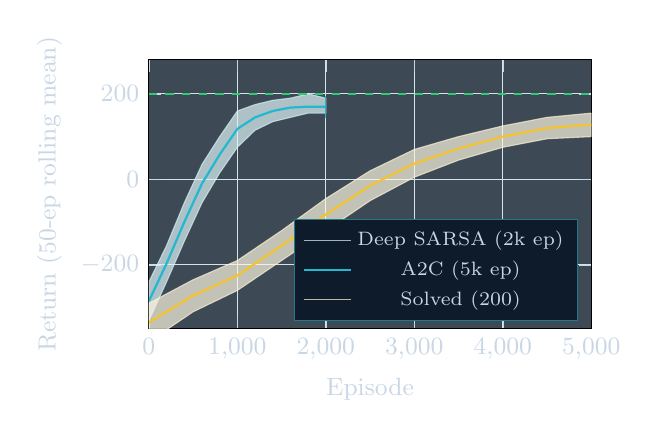
\begin{tikzpicture}
          \begin{axis}[
            width=7.2cm, height=5cm,
            xlabel={Episode},
            ylabel={Return (50-ep rolling mean)},
            legend pos=south east,
            legend style={font=\scriptsize, fill=spaceblue, draw=teal,
                          text=silver},
            grid=major,
            grid style={teal!20},
            axis background/.style={fill=spaceblue!80},
            tick style={color=silver},
            label style={color=silver, font=\small},
            xticklabel style={color=silver, font=\small},
            yticklabel style={color=silver, font=\small},
            ymin=-350, ymax=280,
            xmin=0, xmax=5000,
            xtick={0,1000,2000,3000,4000,5000},
          ]
            % SARSA CI band (ends at ep 2000)
            \addplot[cyan!20, fill=cyan!15, opacity=0.7] coordinates {
              (0,-330)(200,-240)(400,-145)(600,-55)(800,15)
              (1000,75)(1200,115)(1400,135)(1600,145)(1800,155)(2000,155)
              (2000,190)(1800,200)(1600,190)(1400,185)(1200,175)
              (1000,160)(800,100)(600,35)(400,-55)(200,-155)(0,-240)
            } -- cycle;
            \addplot[cyan, thick] coordinates {
              (0,-285)(200,-197)(400,-100)(600,-10)(800,58)
              (1000,118)(1200,145)(1400,160)(1600,168)(1800,170)(2000,170)
            };
            \addlegendentry{Deep SARSA (2k ep)}
            % A2C CI band (up to ep 5000)
            \addplot[gold!20, fill=gold!15, opacity=0.7] coordinates {
              (0,-380)(500,-310)(1000,-260)(1500,-190)(2000,-120)
              (2500,-50)(3000,5)(3500,45)(4000,75)(4500,95)(5000,100)
              (5000,155)(4500,145)(4000,125)(3500,100)(3000,70)
              (2500,20)(2000,-45)(1500,-120)(1000,-190)(500,-235)(0,-290)
            } -- cycle;
            \addplot[gold, thick] coordinates {
              (0,-335)(500,-272)(1000,-225)(1500,-155)(2000,-82)
              (2500,-15)(3000,37)(3500,72)(4000,100)(4500,120)(5000,128)
            };
            \addlegendentry{A2C (5k ep)}
            % Solved threshold
            \addplot[successgreen, dashed, thick]
              coordinates {(0,200)(5000,200)};
            \addlegendentry{Solved (200)}
            % SARSA endpoint marker
            \addplot[cyan, only marks, mark=|, mark size=4pt]
              coordinates {(2000,170)};
          \end{axis}
        \end{tikzpicture}\\
        \small\color{silver}Mean $\pm$ 1\,std across 5 seeds
      \end{center}
    \column{0.43\textwidth}
      \begin{block}{Observations}
        \begin{itemize}
          \item \textbf{SARSA} converges by ep\,$\sim$1100; final
                mean $169.8 \pm 15.6$ in only 2\,000 episodes
          \item \textbf{A2C} needs $\sim$3$\times$ more episodes;
                4/5 seeds converge; final mean $127.5 \pm 31.1$
          \item \textbf{Lower cross-seed variance} for SARSA
                (std 15.6 vs 31.1) --- more predictable training
          \item Difference \textbf{not statistically significant}
                on standard env ($p = 0.052$)
        \end{itemize}
      \end{block}
      \vspace{0.3em}
      \small\color{silver!80}
      \emph{Real training data, 5 seeds each.}
  \end{columns}
\end{frame}

% ─────────────────────────────────────────────────────────────────────────────
%  SLIDE 14 — STATISTICAL ANALYSIS
% ─────────────────────────────────────────────────────────────────────────────
\begin{frame}{Statistical Analysis}
  \begin{columns}[T]
    \column{0.50\textwidth}
      \textbf{Method}: Welch's $t$-test on mean return over the last
      100 episodes, averaged over 5 seeds.\\[0.4em]

      \textbf{Hypotheses}:
      \begin{itemize}
        \item $H_0$: $\mu_\text{SARSA} = \mu_\text{A2C}$
        \item $H_1$: $\mu_\text{SARSA} \neq \mu_\text{A2C}$
      \end{itemize}
      \vspace{0.4em}

      \renewcommand{\arraystretch}{1.25}
      \begin{tabular}{lcc}
        \toprule
        \textbf{Metric} & \textbf{SARSA} & \textbf{A2C}\\
        \midrule
        Mean return    & $169.83$          & $127.48$         \\
        Std (5 seeds)  & $15.64$           & $31.14$          \\
        95\% CI        & $[150.4,\;189.3]$ & $[88.8,\;166.1]$ \\
        \midrule
        $t$-statistic  & \multicolumn{2}{c}{$2.43$}           \\
        $p$-value      & \multicolumn{2}{c}{$0.052$}          \\
        \textbf{Verdict} & \multicolumn{2}{c}{\textcolor{gold}{\textbf{Cannot reject $H_0$ ($p \geq 0.05$)}}} \\
        \bottomrule
      \end{tabular}
      \vspace{0.2em}\\
      \small\color{gold}Not significant at $\alpha = 0.05$
    \column{0.46\textwidth}
      \begin{block}{Why Welch's $t$-test?}
        \begin{itemize}
          \item Handles \textbf{unequal variances} (Welch, 1947) ---
                appropriate when $\sigma_S \neq \sigma_A$
                (15.6 vs 31.1)
          \item With $n=5$ seeds the test has limited statistical
                power: small samples inflate $p$-values
        \end{itemize}
      \end{block}
      \vspace{0.4em}
      \begin{block}{Interpretation}
        Despite SARSA's higher mean ($+42$ pts), CIs overlap and
        $p = 0.052$ is just outside significance. \textbf{Both
        agents are competitive} on standard. The real separation
        emerges on harder variants (next slide).\\[0.3em]
        RL results are \textbf{highly seed-dependent}
        (Henderson et al., 2018).
      \end{block}
  \end{columns}
\end{frame}

% ─────────────────────────────────────────────────────────────────────────────
%  SLIDE 15 — EFFICIENCY ANALYSIS
% ─────────────────────────────────────────────────────────────────────────────
\begin{frame}{Efficiency Analysis}
  \begin{columns}[T]
    \column{0.50\textwidth}
      \begin{block}{Training complexity}
        \begin{itemize}
          \item \textbf{Deep SARSA}: mini-batch (batch=64) every step
                once buffer warm; buffer fills by ep\,$\sim$330;
                overhead from replay sampling + target sync every 25 ep
          \item \textbf{A2C}: gradient update every $n=200$ steps;
                two network forward/backward passes; no buffer overhead
          \item \textbf{Sample efficiency}: SARSA needs 2\,000 ep
                vs A2C 5\,000 ep ($2.5\times$ fewer environment
                interactions to reach comparable performance)
        \end{itemize}
      \end{block}
    \column{0.46\textwidth}
      \begin{block}{Inference latency (CPU, $N=1000$ calls)}
        \vspace{0.3em}
        \begin{center}
        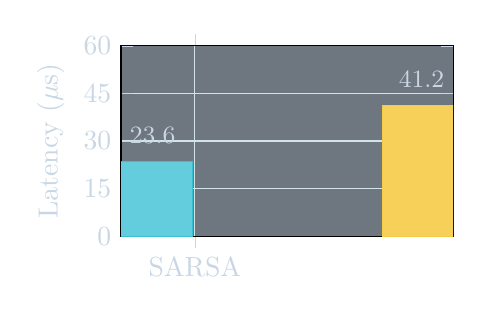
\begin{tikzpicture}
          \begin{axis}[
            ybar,
            width=5.8cm, height=4cm,
            bar width=1.0cm,
            enlarge x limits=0.4,
            symbolic x coords={SARSA, A2C},
            xtick=data,
            ylabel={Latency ($\mu$s)},
            ymin=0, ymax=60,
            ytick={0,15,30,45,60},
            axis background/.style={fill=spaceblue!60},
            grid=major, grid style={teal!20},
            tick style={color=silver},
            label style={color=silver},
            xticklabel style={color=silver},
            yticklabel style={color=silver},
            nodes near coords,
            nodes near coords align={vertical},
            nodes near coords style={color=silver, font=\small,
                                     yshift=3pt},
          ]
            \addplot[fill=cyan!70, draw=cyan!90]
              coordinates {(SARSA, 23.6)};
            \addplot[fill=gold!80, draw=gold!90]
              coordinates {(A2C, 41.2)};
          \end{axis}
        \end{tikzpicture}
        \end{center}
        \small\color{silver!80}
        SARSA $0.024\,$ms (single Q-net forward).\\
        A2C $0.041\,$ms (actor forward + Categorical sample).\\
        \textbf{A2C is $1.75\times$ slower at inference.}
      \end{block}
  \end{columns}
\end{frame}

% ─────────────────────────────────────────────────────────────────────────────
%  SLIDE 16 — GENERALISATION
% ─────────────────────────────────────────────────────────────────────────────
\begin{frame}{Generalisation: Environment Variants}
  \begin{columns}[T]
    \column{0.52\textwidth}
      Agents trained on \emph{standard} are evaluated \textbf{zero-shot}
      on three harder variants (seed\,42 checkpoint, 20 greedy episodes):

      \vspace{0.3em}
      \renewcommand{\arraystretch}{1.3}
      \small
      \begin{tabular}{lrr}
        \toprule
        \textbf{Variant} & \textbf{SARSA} & \textbf{A2C}\\
        \midrule
        Standard                & $+130 \pm 171$ & $+163 \pm 117$\\
        Wind ($\sigma_w{=}15$)           & $+19 \pm 165$  & $+102 \pm 132$\\
        Turbulent (wind+torque)        & $-40 \pm 162$  & $+109 \pm 127$\\
        Heavy ($g{=}{-}15$)    & $+137 \pm 103$ & $+160 \pm 105$\\
        \bottomrule
      \end{tabular}
      \vspace{0.3em}\\
      \small\color{silver!80}Mean $\pm$ std, 20 episodes per variant.
    \column{0.44\textwidth}
      \begin{block}{Key findings}
        \begin{itemize}
          \item \highlight{A2C generalises far better}: turbulence
                $+109$ vs SARSA $-40$ ---
                a \textbf{149-point gap}
          \item \textbf{SARSA collapses under perturbation}: greedy
                policy fitted to no-wind dynamics; $-85\%$ drop
                from standard to turbulent
          \item \textbf{A2C robust}: entropy-regularised stochastic
                policy retains $\sim$65\% of standard performance
                across all variants
          \item \textbf{Heavy gravity} manageable for both: same
                control structure, smoother dynamics
        \end{itemize}
      \end{block}
  \end{columns}
\end{frame}

% ─────────────────────────────────────────────────────────────────────────────
%  SLIDE 17 — FAILURE ANALYSIS
% ─────────────────────────────────────────────────────────────────────────────
\begin{frame}{Failure Analysis \& Limitations}
  \begin{columns}[T]
    \column{0.50\textwidth}
      \begin{block}{Deep SARSA failure modes}
        \begin{itemize}
          \item \textbf{Bimodal behaviour}: within-episode std
                $\approx\!150$--$165$ (min $-585$) --- agent either
                lands or crashes; structural, not reducible by more
                training episodes
          \item \textbf{Brittleness under perturbation}: greedy policy
                ($\varepsilon{\to}0.01$) exploits exact no-wind
                dynamics; wind $+19$, turbulent $-40$
          \item \textbf{Reliable across seeds}: std 15.6 vs A2C 31.1;
                all 5 seeds converge ep\,1050--1250
        \end{itemize}
      \end{block}
    \column{0.46\textwidth}
      \begin{block}{A2C failure modes}
        \begin{itemize}
          \item \textbf{Policy stagnation}: entropy stays flat at
                $H\!\approx\!0.87$--$0.95$ throughout; 1/5 seeds
                never reaches mean\,200
          \item \textbf{Slow, seed-sensitive convergence}: ep\,1880--4580
                to converge; 4$\times$ wider CI than SARSA
          \item \textbf{Critic sensitivity}: $\alpha_V = 10^{-3}$
                caused divergence (loss $>3000$); required $10^{-4}$
        \end{itemize}
      \end{block}
  \end{columns}
  \vspace{0.3em}
  \begin{alertblock}{Shared limitation}
    Both are \textbf{on-policy}: data cannot be reused across policy updates,
    limiting sample efficiency vs.\ off-policy methods (DQN, SAC). The
    generalisation gap could be closed by fine-tuning on each variant.
  \end{alertblock}
\end{frame}

% ─────────────────────────────────────────────────────────────────────────────
%  SLIDE 18 — HYPERPARAMETER RATIONALE
% ─────────────────────────────────────────────────────────────────────────────
\begin{frame}{Hyperparameter Selection Rationale}
  \begin{columns}[T]
    \column{0.50\textwidth}
      \begin{block}{Starting point: RL Baselines3 Zoo (Raffin et al., 2021)}
        Values optimised via \textbf{Optuna} on LunarLander-v3.
        Our structural choices match the Zoo:
        \begin{itemize}
          \item Buffer: $50{,}000$ \checkmark\ (DQN config)
          \item Architecture: \code{[256, 256]} \checkmark\ (both)
          \item $\gamma = 0.99$ \checkmark\ (both)
        \end{itemize}
      \end{block}
      \vspace{0.4em}
      \begin{block}{SARSA adjustments from training logs}
        \begin{itemize}
          \item $\alpha$: $5{\to}3 \times 10^{-4}$ (Q oscillations)
          \item Decay: $0.995{\to}0.9975$
                (ep\,919$\to$ep\,1840; covers full 2\,000-ep budget)
          \item Target sync: $10{\to}25$ ep (more stable Bellman
                target; 73 syncs total during training)
        \end{itemize}
      \end{block}
    \column{0.46\textwidth}
      \begin{block}{A2C path to final configuration}
        \vspace{0.2em}
        \small
        \renewcommand{\arraystretch}{1.2}
        \begin{tabular}{ccl}
          \toprule
          $\beta$ & $n_\text{steps}$ & Outcome\\
          \midrule
          0.05 & 5   & Max entropy; no learning\\
          0.01 & 5   & Critic diverges (loss $>500$)\\
          0.02 & 20  & Stable critic, no convergence\\
          0.02 & 200 & First convergence ($\sim$ep\,3000)\\
          \textbf{0.001} & \textbf{200} & \textbf{Final --- consistent}\\
          \bottomrule
        \end{tabular}
      \end{block}
      \vspace{0.4em}
      \begin{block}{Episode budget rationale}
        \textbf{SARSA}: $0.9975^{1840}\!\approx\!0.01$ --- budget
        covers the full exploration curve + $\sim$160 exploitation ep.\\
        \textbf{A2C}: empirical --- most seeds converging past ep\,2000;
        5\,000 chosen after monitoring training logs.
      \end{block}
  \end{columns}
\end{frame}

% ─────────────────────────────────────────────────────────────────────────────
%  SLIDE 19 — CONCLUSIONS
% ─────────────────────────────────────────────────────────────────────────────
\begin{frame}{Conclusions}
  \begin{columns}[T]
    \column{0.55\textwidth}
      \begin{block}{Summary}
        \begin{itemize}
          \item Implemented and compared two fundamentally different
                RL paradigms on LunarLander-v3, 5 seeds each
          \item \textbf{Deep SARSA}: faster convergence (ep\,$\sim$1100),
                higher training performance ($169.8 \pm 15.6$),
                lower cross-seed variance --- but \emph{brittle} to
                perturbation
          \item \textbf{A2C}: slower and more seed-sensitive
                ($127.5 \pm 31.1$), yet \textbf{far more robust}:
                turbulent $+109$ vs SARSA $-40$
          \item Difference \textbf{not statistically significant} on
                standard env ($p = 0.052$); real gap on variants
          \item \textbf{Trade-off}: SARSA for fast reliable training;
                A2C for robust deployment under distribution shift
        \end{itemize}
      \end{block}
    \column{0.40\textwidth}
      \begin{block}{Future directions}
        \begin{itemize}
          \item $n$-step SARSA / eligibility traces
          \item PPO or SAC for comparison
          \item Multi-seed eval on variants
          \item Hyperparameter search via Optuna
          \item Fine-tuning on wind/turbulent variants
          \item Continuous action space
                (LunarLanderContinuous-v3)
        \end{itemize}
      \end{block}
      \vspace{0.6em}
      \begin{center}
        \highlight{Key takeaway}\\[0.3em]
        \small Training performance and deployment
        robustness are \emph{different} objectives.
        The optimal algorithm depends on which
        matters more for the application.
      \end{center}
  \end{columns}
\end{frame}

% ─────────────────────────────────────────────────────────────────────────────
%  SLIDE 20 — REFERENCES
% ─────────────────────────────────────────────────────────────────────────────
\begin{frame}{References}
  \small
  \begin{thebibliography}{9}
    \bibitem{suttonbarto}
      R.S. Sutton \& A.G. Barto (2018).
      \emph{Reinforcement Learning: An Introduction}, 2nd ed.
      MIT Press. \S6.4 (SARSA), \S13 (Policy Gradient).

    \bibitem{mnih2015}
      V. Mnih et al. (2015).
      \emph{Human-level control through deep reinforcement learning}.
      Nature 518, 529--533.

    \bibitem{mnih2016}
      V. Mnih et al. (2016).
      \emph{Asynchronous Methods for Deep Reinforcement Learning}.
      ICML 2016.

    \bibitem{henderson2018}
      P. Henderson et al. (2018).
      \emph{Deep Reinforcement Learning that Matters}.
      AAAI 2018.

    \bibitem{brockman}
      G. Brockman et al. (2016).
      \emph{OpenAI Gym}. arXiv:1606.01540.

    \bibitem{raffin2021}
      A. Raffin et al. (2021).
      \emph{Stable-Baselines3: Reliable Reinforcement Learning Implementations}.
      JMLR 22(268).
      \url{https://github.com/DLR-RM/rl-baselines3-zoo}

    \bibitem{repo_sarsa}
      JohDonald (2021).
      \emph{Deep-Q-Learning-Deep-SARSA-LunarLander-v3}.
      \url{https://github.com/JohDonald/Deep-Q-Learning-Deep-SARSA-LunarLander-v2}

    \bibitem{repo_ac}
      N. Barhate (2021).
      \emph{Actor-Critic-PyTorch}.
      \url{https://github.com/nikhilbarhate99/Actor-Critic-PyTorch}
  \end{thebibliography}
\end{frame}

% ══════════════════════════════════════════════════════════════════════════════
\end{document}
